%!TEX root = toolhinweise.tex

% Document Class
\documentclass{../../../template/exercise-document-de}

% Exercise Properties
\newcommand{\docLectureName}{\red{LEHRVERANSTALTUNG}}
\newcommand{\docLectureTime}{\red{JAHR/SEMESTER}}
\newcommand{\docLectureHost}{\red{DOZENT:INNEN}}

\newcommand{\docAssignmentNumber}{\red{1}}
\newcommand{\docAssignmentTitle}{\red{TITEL DER AUFGABE}}
\newcommand{\docTitle}{Toolhinweise}

\setcounter{tocdepth}{3}

% Content
\begin{document}
	\maketitle

	\red{Stand: 26.07.2022}
	
	\setcounter{tocdepth}{2}
	\tableofcontents

	\newpage
	%!TEX root = ../toolhinweise.tex

\section{Installation und Konfiguration}
\label{sec:installation}


\textbf{YAKINDU Statechart Tools (SCT)} ist ein Eclipse-Plugin.
Da es gelegentlich zu Problemen mit einem nachinstallierten Plugin kommt, empfehlen wir YAKINDU SCT als separates Standalone-Programm zu installieren. 

Für die Kombination von YAKINDU SCT mit dem für das \docProjectTitle{} gegebenen Validierungsframework wird ein \textbf{Java Development Kit (JDK)} mit \textbf{mindestens Version 10} benötigt (getestet mit den Versionen 10.0.2, 11.0.2, 12.0.1 und 17.0.2 LTS und 18.0.1.1). In dieser Installationsanleitung wird die neuste Version Java 18.0.1.1 verwendet und YAKINDU SCT 4.0.





%%%%%%%%%%%%%%%%%%%%%%%%%%%%%%%%%%%%%%%%%%%%%%%%%%%%%%%%%%%%%%%%%%%%%%%%%%%%%%%%%%%%%%%%%%%%%%%%%%%%%%%%%%%%%%%%%%%





\subsection{JDK und YAKINDU SCT installieren}

\subsubsection{Windows 10}

\begin{enumerate}
	\setlength\topsep{-1em}
	\setlength\itemsep{-0.5em}
	\item Java herunterladen (auf der Webseite die .exe-Datei auswählen):
	\\\url{https://www.oracle.com/java/technologies/downloads/#jdk18-windows}
	\item Java gemäß den Anweisungen installieren.
	\item Falls noch nicht automatisch erfolgt, Java zur System-Path-Variable hinzufügen:
	\vspace{-0.5em}
	\begin{enumerate}
		\setlength\itemsep{-0.5em}
		\item In der Suchleiste \enquote{Systemumgebungsvariablen bearbeiten} suchen und öffnen.
		\item Den Button \enquote{Umgebungsvariablen} anklicken. 
		\item Die Variable \enquote{Path} im unteren Bereich \enquote{Systemvariablen} auswählen und \enquote{Bearbeiten} klicken. 
		\item Falls Java noch nicht eingetragen ist, hier den Pfad der neuen Java-Installation hinzufügen (z.B. \texttt{C:\textbackslash{}Program Files\textbackslash{}Java\textbackslash{}jdk-17.0.2\textbackslash{}bin}).
	\end{enumerate}
	\item YAKINDU Statechart Tools Professional für \enquote{Windows 64 Bit} Edition herunterladen:
	\\\url{https://www.itemis.com/en/yakindu/state-machine/download-options/}
	\item Heruntergeladene .zip-Datei an einem beliebigen Ort entpacken.
	\item Nachdem die .zip-Datei entpackt wurde, im entpackten Ordner die Datei \texttt{SCT.exe} ausführen.
\end{enumerate}

\subsubsection{MacOS X}

\begin{enumerate}
	\setlength\topsep{-1em}
	\setlength\itemsep{-0.5em}
	\item Java herunterladen (auf der Webseite die .dmg-Datei für die entsprechende Architektur auswählen):
	\\\url{https://www.oracle.com/java/technologies/downloads/#jdk18-mac}
	\item Java gemäß den Anweisungen installieren.
	\item YAKINDU Statechart Tools Professional für \enquote{macOS X 64 Bit} Edition herunterladen:
	\\\url{https://www.itemis.com/en/yakindu/state-machine/download-options/}
	\item Heruntergeladene \texttt{YAKINDU SCTPRO.app} in den Ordner Programme verschieben und starten.
\end{enumerate}



\subsubsection{Linux}

Die Installation auf Linux wurde mit Ubuntu Versionen 18.10, 19.04 und 20.04 getestet. Bei anderen Distributionen ergeben sich ggf. Abweichungen.


\subsubsection*{Variante 1: JDK über PPA beziehen}
\begin{enumerate}
	\setlength\topsep{-1em}
	\setlength\itemsep{-0.5em}
	\item \texttt{sudo add-apt-repository ppa:linuxuprising/java}
	\item \texttt{sudo apt-get update}
	\item \texttt{sudo apt-get install oracle-java18-installer}
	\item Falls mehrere Java-Versionen installiert sind: \\\texttt{sudo apt-get install oracle-java18-set-default}
	\item Installation mit \texttt{javac -version} prüfen.
\end{enumerate}



\subsubsection*{Variante 2: JDK direkt herunterladen}
\begin{enumerate}
	\setlength\topsep{-1em}
	\setlength\itemsep{-0.5em}
	\item Java herunterladen:
	\\\url{https://www.oracle.com/java/technologies/downloads/#jdk18-linux}
	\item Zur manuellen Java-Installation von Java aus einer .tar.gz-Datei diese entpacken und den Anweisungen der beiliegenden \texttt{README}-Datei folgen.
\end{enumerate}


\subsubsection*{Beide Varianten: YAKINDU SCT installieren}
\begin{enumerate}
	\setlength\topsep{-1em}
	\setlength\itemsep{-0.5em}
	\item YAKINDU Statechart Tools Professional für \enquote{Linux 64 Bit} Edition herunterladen:
	\\\url{https://www.itemis.com/en/yakindu/state-machine/download-options/}
	\item Heruntergeladene .zip-Datei an einem beliebigen Ort entpacken.
	\item Nachdem die .zip-Datei entpackt wurde, im entpackten Ordner die Datei \enquote{\texttt{SCT}} als ausführbar markieren und starten.
\end{enumerate}




%%%%%%%%%%%%%%%%%%%%%%%%%%%%%%%%%%%%%%%%%%%%%%%%%%%%%%%%%%%%%%%%%%%%%%%%%%%%%%%%%%%%%%%%%%%%%%%%%%%%%%%%%%%%%%%%%%%




\subsection{YAKINDU SCT aktivieren}

Für Mitarbeiter und Studierende des Hasso-Plattner-Instituts steht eine akademische Lizenz für die Professional Edition von YAKINDU SCT zur Verfügung.
Für die Bearbeitungsdauer vom \docProjectTitle{} genügt unter Umständen aber auch die automatisch vorinstallierte 30-Tage Probelizenz.



\subsubsection*{Akademischen Lizenz beantragten}

Auf der folgenden Webseite kann mit Angabe einer Universitäts-Email-Adresse eine kostenlose akademische Lizenz beantragt werden:

\begin{center}
	\url{https://www.itemis.com/en/yakindu/state-machine/licenses#professional-edition-academic-license}
\end{center}


In der Regel dauert es 1 Tag bis zur Freigabe. Es kann nach Ablauf der Lizenz mit der selben Email-Adresse eine neue beantragt werden.



\subsubsection*{Einbinden der akademischen Lizenz}

\begin{enumerate}
	\setlength\topsep{-1em}
	\setlength\itemsep{-0.5em}
	\item YAKINDU SCT zeigt zuerst einen \enquote{Welcome Screen} an. Diesen schließen.
	\item Im Menü unter \enquote{Window} das Fenster \enquote{Preferences} öffnen.
	\item Dort \enquote{YAKINDU Licences} (vorletzter Punkt) auswählen.
	\item Auf \enquote{Import License File...} klicken.
	\item Die per E-Mail erhaltene Datei auswählen.
	\item Bestätigen und das Einstellungsfenster schließen.
\end{enumerate}





%%%%%%%%%%%%%%%%%%%%%%%%%%%%%%%%%%%%%%%%%%%%%%%%%%%%%%%%%%%%%%%%%%%%%%%%%%%%%%%%%%%%%%%%%%%%%%%%%%%%%%%%%%%%%%%%%%%





\subsection{\enquote{\red{PROJEKTNAME}}-Projekt einrichten}
\label{subsec:import}

\subsubsection{Projektdaten beziehen}

Das \enquote{\red{PROJEKTNAME}}-Projekt wird über \red{HIER LINK ZUM REPOSITORY} bereitgestellt.
Es wird empfohlen das Repository zu forken, um stets aktuelle Updates zu erhalten.
In dem Repository können zudem Issues gemeldet werden.

% Der aktuelle Stand des Repositories wird zudem als .zip-Archiv im Moodle bereitgestellt.


\subsubsection{\enquote{\red{PROJEKTNAME}}-Projekt in YAKINDU SCT importieren}


Das Repository beinhaltet einen Eclipse-Projektordner, der in YAKINDU SCT importiert werden kann.

\begin{enumerate}
	\setlength\topsep{-1em}
	\setlength\itemsep{-0.5em}
	\item Den Projektordner (über das Repository oder die .zip-Datei im Moodle) auf der Festplatte speichern.
	\item YAKINDU SCT, wie oben beschrieben, starten und den \enquote{Welcome Screen} schließen.
	\item Links im \enquote{Project Explorer} einen Rechtsklick machen und \enquote{Import} auswählen.
	\item Dort \enquote{General} $\rightarrow$ \enquote{Existing Projects into Workspace} auswählen.
	\item Dann oben rechts auf \enquote{Directory} klicken und Projektordner auswählen.
	\item In der Projektliste sollte ein Projekt mit dem Namen \enquote{mod2-2022-sctsim} angezeigt werden. Dieses auswählen.
	\item Auf \enquote{Finish} klicken, um den Import abzuschließen. Das Projekt ist jetzt links im \enquote{Project Explorer} verfügbar.
\end{enumerate}



\subsection{Problembehebung}

Das vorgegebene Eclipse-Projekt enthält alle notwendigen Einstellungen und sollte in den meisten Fällen direkt benutzbar sein.

Es kann allerdings passieren, dass lokale Einstellungen (z.B. die installierte Java-Version) Teile der Projektkonfiguration überschreiben. In diesem Fall können die relevanten Einstellungen manuell geändert werden.
Dies ist auch notwendig, wenn, anstatt ein Projekt zu importieren (wie im \autoref{subsec:import} beschrieben), ein neues Eclipse-Projekt angelegt wird.

Zum Anpassen der Projekteinstellungen kann im \enquote{Project Explorer} das \enquote{mod2-2022-sctsim}-Projekt mit einem Rechtsklick angeklickt und \enquote{Properties} ausgewählt werden.

\enlargethispage{1\baselineskip}

\subsubsection{Java-Version manuell festlegen} 

Ist keine oder eine falsche Version von Java eingebunden, kann dies in den Projekteinstellungen geändert werden.


\begin{figure}
	\centering
	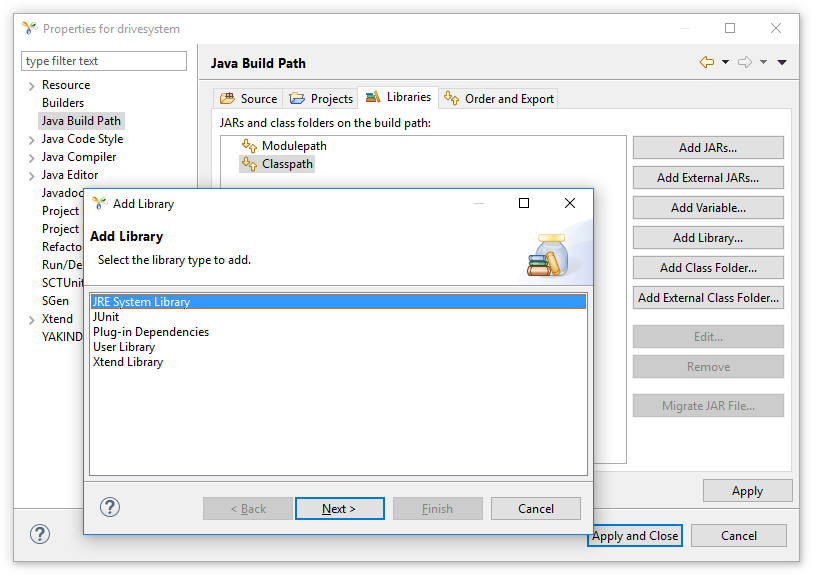
\includegraphics[width=0.7\textwidth]{yakindu_java_version}
	\caption{In den Projekteinstellungen kann eine bestimmte JRE-Version festgelegt werden}
	\label{fig:yakindu_java}
\end{figure}

In den Einstellungen wird dazu \enquote{Java Build Path} ausgewählt und dort der Tab \enquote{Libraries} geöffnet. Mit dem Button \enquote{Add Library...} kann eine \enquote{JRE System Library} hinzugefügt werden (siehe \autoref{fig:yakindu_java}).
Falls in der Liste bereits ein JRE-Eintrag vorkommt, kann dieser per \enquote{Edit...} angepasst werden. 
Mit einem Klick auf \enquote{Installed JREs...} kann die Liste der Eclipse bekannten Java-Versionen eingesehen und bearbeitet werden.

In manchen Fällen muss neben dem JRE-Eintrag auch noch ein JUnit-Eintrag hinzugefügt werden. 
Dabei muss JUnit Version 4 ausgewählt werden.

In seltenen Fällen wird nach dem Ändern der Java-Version an einigen Stellen im Code das Keyword \texttt{var} weiterhin als Fehler erkannt. 
Um dies zu vermeiden, bietet Eclipse als Korrekturvorschlag an, die \enquote{Project compliance} auf die neue Java-Version zu setzen. 
Zum Nutzen eines Korrekturvorschlags kann auf eine der Fehlermeldungen im \enquote{Problems}-Fenster oder an der entsprechend markierten Stelle im Code rechts geklickt werden.




\subsubsection{Projektordner manuell festlegen}

Wenn beim Programmstart Dateien nicht gefunden werden können, könnte es sinnvoll sein, die Liste der eingebundenen Quelltextordner in den Projekteinstellungen zu kontrollieren.


\begin{figure}
	\centering
	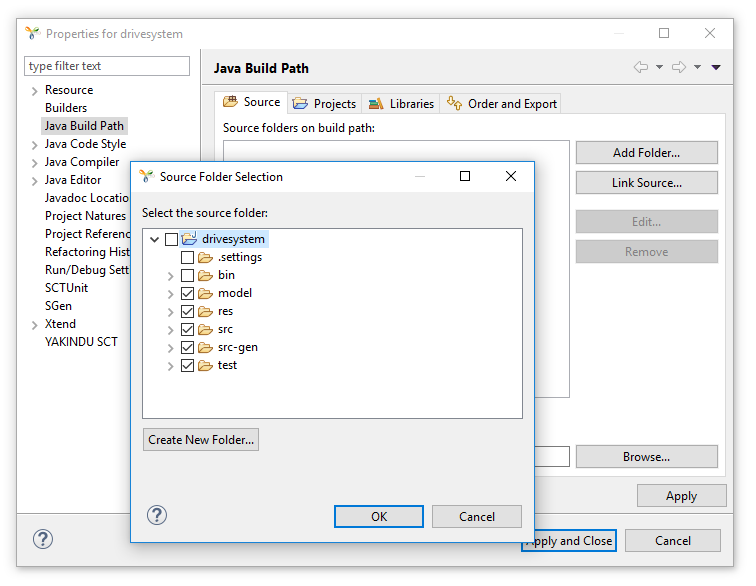
\includegraphics[width=0.7\textwidth]{yakindu_folders}
	\caption{In den Projekteinstellungen können die vom Eclipse-Projekt eingebundenen Quelltextordner festgelegt werden}
	\label{fig:yakindu_folders}
\end{figure}

Dazu wird in den Einstellungen der \enquote{Java Build Path} ausgewählt und dort der Tab \enquote{Source} geöffnet. 
Mit dem Button \enquote{Add Folder...} können nun Ordner hinzugefügt werden  (siehe \autoref{fig:yakindu_folders}).
Es müssen die Ordner \texttt{model}, \texttt{res}, \texttt{src}, \texttt{src-gen} und \texttt{test} ausgewählt werden.

\enlargethispage{1\baselineskip}


\subsubsection{Eclipse-Projekt umbenennen} 

In seltenen Fällen vergibt YAKINDU SCT dem \enquote{mod2-2022-sctsim}-Projekt beim Importieren einen anderen Namen (wie z.B. \enquote{mod2-2022-sctsim-master}).
In diesen Fällen muss das importierte Projekt umbenannt werden, da für die Codegenerierung der Projektname unbedingt \enquote{mod2-2022-sctsim} lauten muss. 
Zum Umbenennen muss im \enquote{Project Explorer} rechts auf das Projekt geklickt werden und \enquote{Refactor} $\rightarrow$ \enquote{Rename} ausgewählt werden.


	
	\newpage
	%!TEX root = ../toolhinweise.tex

\section{YAKINDU Statechart Syntax}
\label{sec:syntax}

Statecharts können die gleichen Konstrukte abbilden wie UML Zustandsdiagramme.
YAKINDU SCT zielt auf die Ausführung von Statecharts ab und erzwingt deswegen eine präzisere und striktere Syntax, damit die Ausführung in jedem Fall eindeutig ist. 

Hier werden die wichtigsten Besonderheiten vorgestellt. Eine vollständige Spachreferenz befindet sich auf \url{https://www.itemis.com/en/yakindu/state-machine/documentation/user-guide/sclang_statechart_language_reference}.

\subsection{Zustände und Regionen}

Statecharts bestehen aus Regionen, die Zustände beinhalten können, die wiederum Regionen beinhalten können, die neue Zustände beinhalten können, und so weiter. Regionen werden dargestellt als hellgraue Rechtecke, Zustände als hellblaue abgerundete Rechtecke. 
Regionen können wie Zustände Namen haben, die Benennung ist aber optional. 
Ein Zustand, der Regionen beinhaltet, kann dennoch lokale Reaktionen haben. 
Wenn innerhalb eines Zustandes mehrere (orthogonale) Regionen sind müssen Sie eine explizite (Ausführungs-)Reihenfolge haben.

\begin{center}
	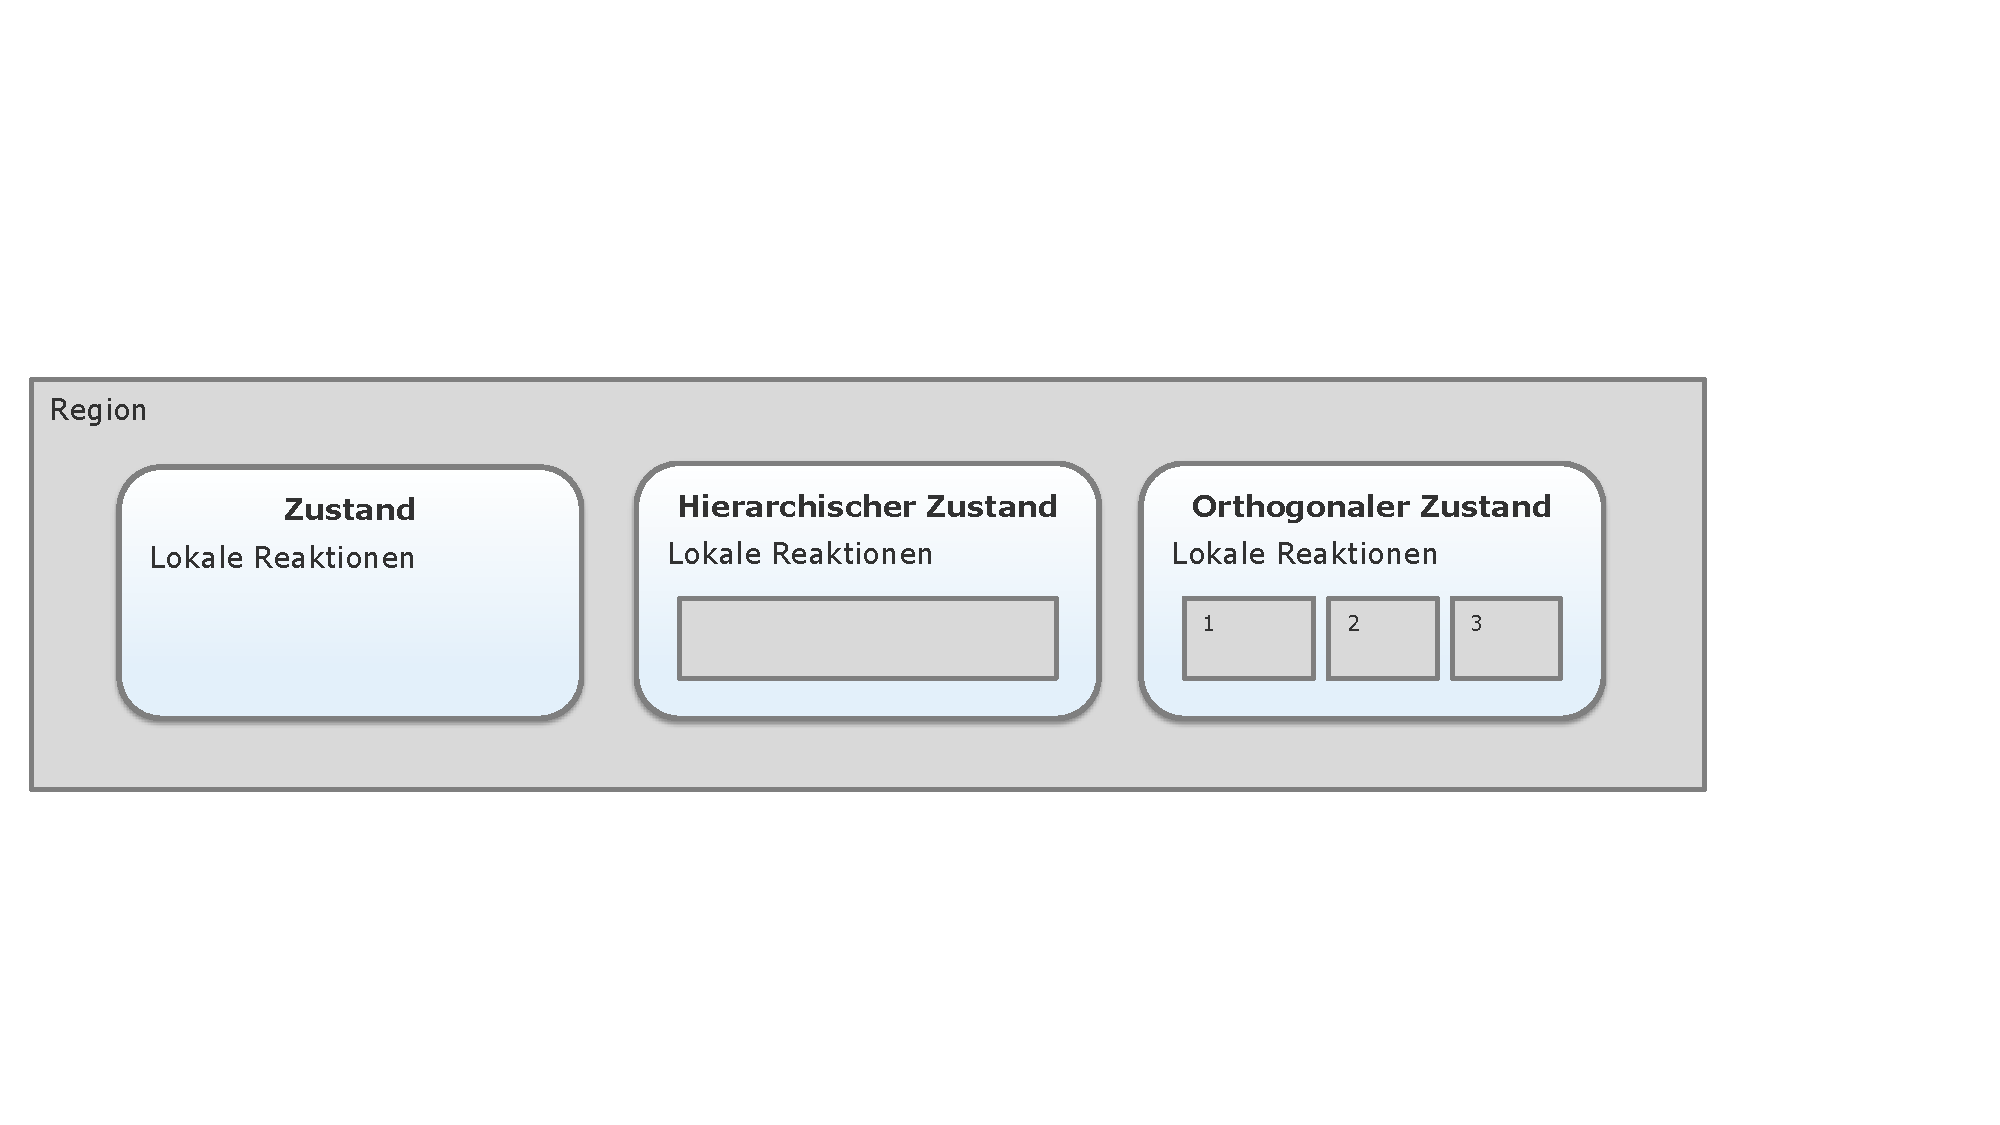
\includegraphics[width=0.8\textwidth]{syntax_regionen}
\end{center}

Bei UML-Zustandsdiagrammen sind Regionen ebenfalls Teil der Spezifikation und Logik, sind aber nicht Teil der konkreten Syntax und werden daher nicht explizit graphisch mitmodelliert.


\subsection{Reaktionen}

Alles Verhalten in einem Statechart wird durch Reaktionen beschreiben, die in Zuständen oder an Transitionen stehen. 
Eine Reaktion besteht aus einem Trigger (\emph{Eingabe}), eventuell einem Guard (\emph{Bedingung} in eckigen Klammern) und eventuell Effekten (\emph{Ausgaben} und \emph{Seiteneffekte}). 

Trigger und Guards funktionieren wie in UML-Zustandsdiagrammen.
Zu beachten ist nur, dass \enquote{else} im Statechart ein Trigger statt ein Guard ist und deshalb nicht in eckigen Klammern steht.

Wie bei einem UML-Zustandsdiagramm werden Effekte immer mit einem \enquote{/} vom vorderen Teil der Reaktion getrennt. Mehrere Effekte werden voneinander mit \enquote{;} getrennt.
Besonderheit bei den Effekten ist, dass ausgehenden Ereignissen (\emph{Ausgaben}) das Schlüsselwort \enquote{raise} vorangestellt werden muss.

Alle in einem Zustand möglichen Reaktionen haben eine feste Ausführungsreihenfolge. Die internen Reaktionen werden von oben nach unten ausgeführt, die ausgehenden Transitionen aus einem Zustand sind explizit nummeriert, genauso wie die Transitionen die auf eine Verzweigung folgen.

\begin{center}
	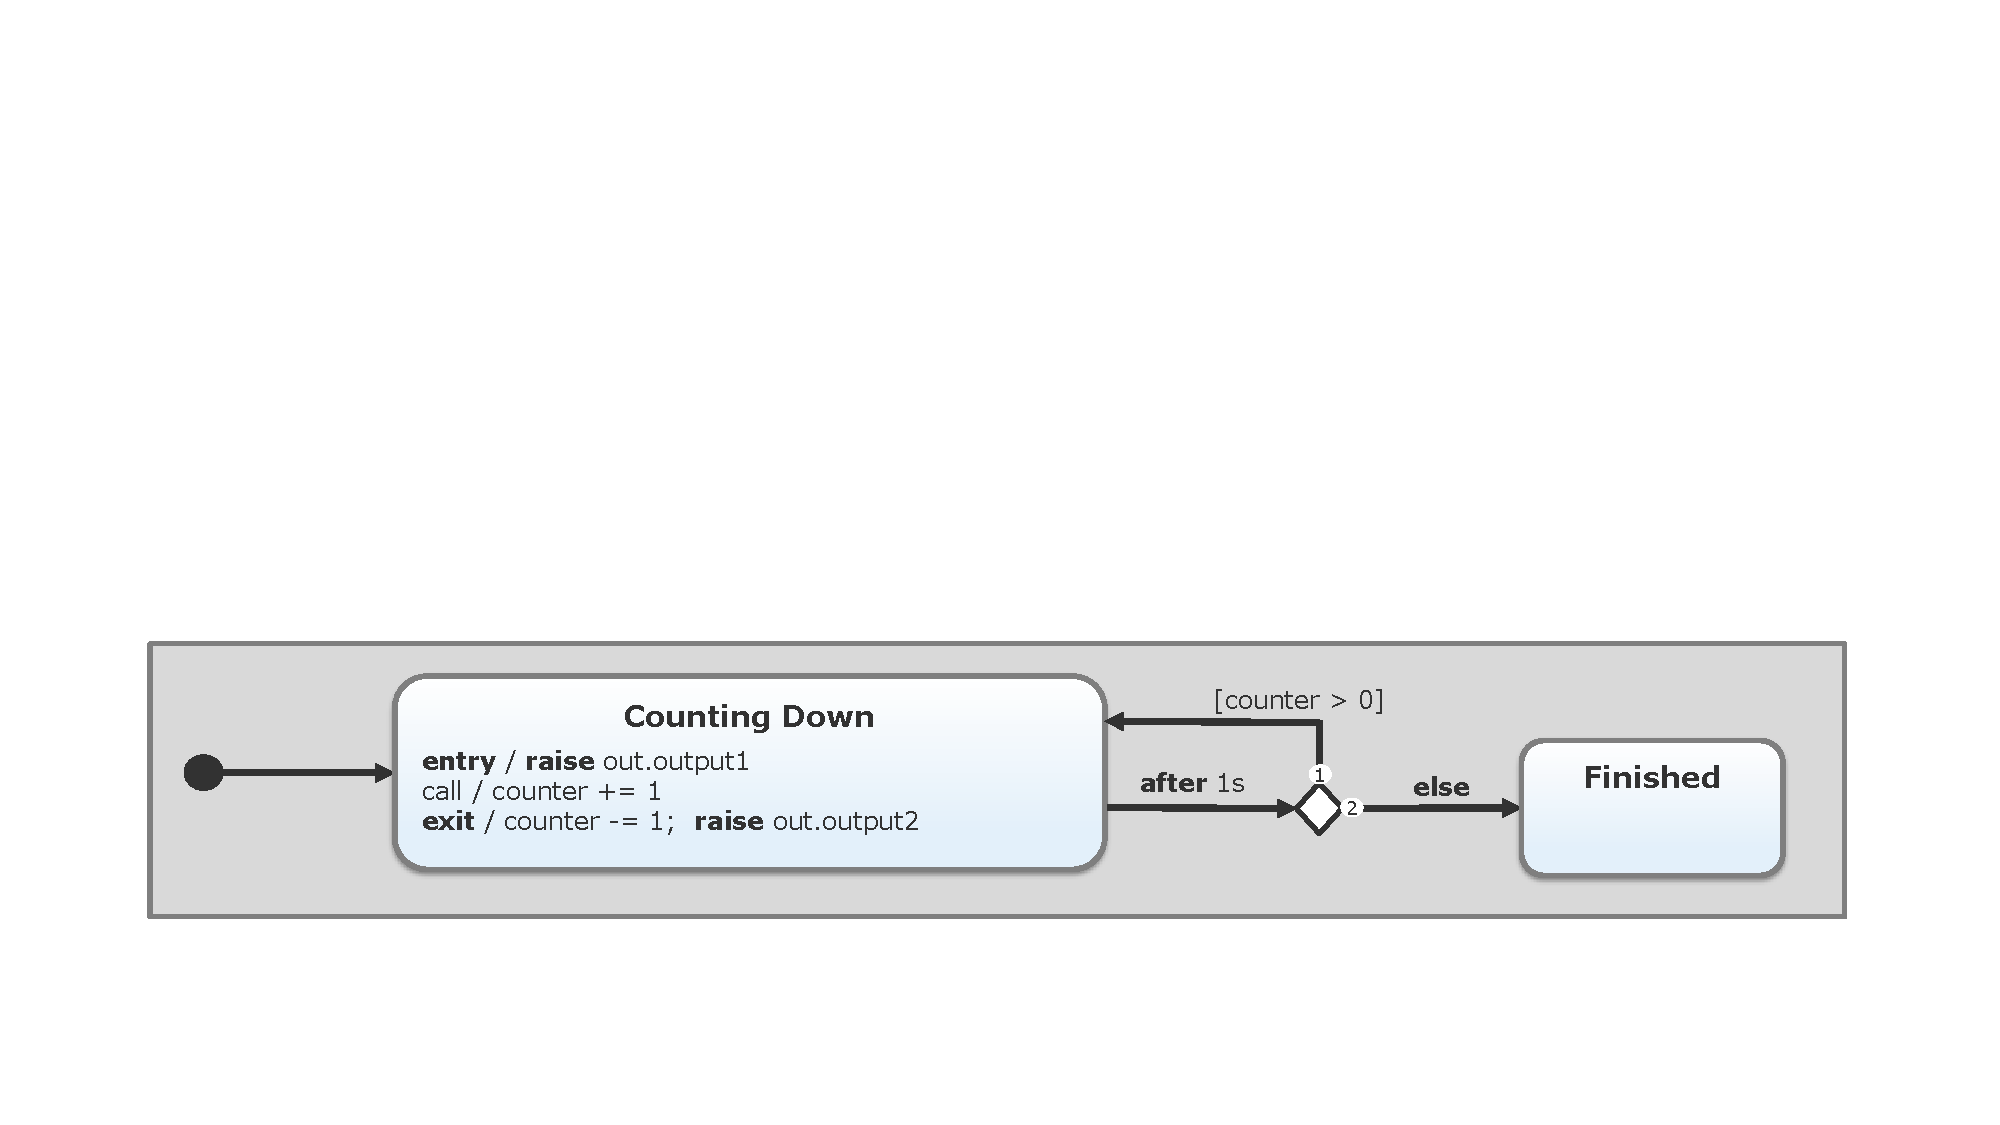
\includegraphics[width=1\textwidth]{syntax_reaktionen}
\end{center}



\subsection{Definitionsbereich}

Ein YAKINDU Statechart hat einen zusätzlichen Definitionsbereich, in dem alle für die Reaktionen benötigten Elemente definiert werden können. Das beinhaltet insbesondere eingehende und ausgehende Ereignisse sowie Operationen, die beispielsweise in Guards aufgerufen werden können. 
Dies entspricht in etwa dem Ein- und Ausgabealphabet eines erweiterten Automaten bzw. dem Klassendiagramm zu einem UML-Zustandsdiagramm. Für diese Aufgabenstellung ist der entsprechende Teil des Definitionsbereiches fest vorgegeben und \textbf{darf nicht verändert werden}.

Außerdem können im Definitionsbereich interne Ereignisse (die per \enquote{raise} aufgerufen und als Trigger empfangen werden können) zur Synchronisation sowie interne Variablen definiert werden.
Dieser mit \enquote{internal} markierte Teil des Definitionsbereiches darf für die Lösung von \docProjectTitle{} um eigene Ereignisse und Variablen ergänzt werden.

Der Definitionsbereich ermöglicht YAKINDU SCT die strikte Syntaxprüfung bei den Reaktionen.


	\newpage
	%!TEX root = ../toolhinweise.tex

\section{Nutzung von YAKINDU SCT}
\label{sec:yakindu}

In diesem Abschnitt werden ergänzend zur Vorstellung der Syntax-Besonderheiten in \autoref{sec:syntax} einige Hinweise zur Nutzung von YAKINDU SCT gegeben.

Eine detaillierte Erläuterung zu YAKINDU SCT findet sich unter \url{https://www.itemis.com/en/yakindu/state-machine/documentation/user-guide/edit_editing_statecharts}.

\enlargethispage{1\baselineskip}




%%%%%%%%%%%%%%%%%%%%%%%%%%%%%%%%%%%%%%%%%%%%%%%%%%%%%%%%%%%%%%%%%%%%%%%%%%%%%%%%%%%%%%%%%%%%




\subsection{Nutzung von Versionskontrollsystemen}

Ein Statechart in YAKINDU SCT ist in einer einzigen .sct-Datei gespeichert. 
Die .sct-Dateien können \emph{nicht} gemergt werden. 
Bei der Verwendung eines Versionskontrollsystems (z.B. Git) ist also auf die Vermeidung von Konflikten zu achten.

Wenn parallel auf verschiedenen Geräten an verschiedenen Statechart-Features gearbeitet wird, besteht die Möglichkeit, eine der .sct-Dateien (und die dazugehörige .sgen-Datei) umzubenennen. 
Die Codegenerierung ist so weiterhin möglich. 
Zum Zusammenführen der .sct-Dateien ist es in YAKINDU SCT möglich Diagrammelemente zwischen diesen Dateien zu kopieren.




%%%%%%%%%%%%%%%%%%%%%%%%%%%%%%%%%%%%%%%%%%%%%%%%%%%%%%%%%%%%%%%%%%%%%%%%%%%%%%%%%%%%%%%%%%%%




\subsection{Modellierung von Statecharts}

\begin{figure}[t]
	\centering
	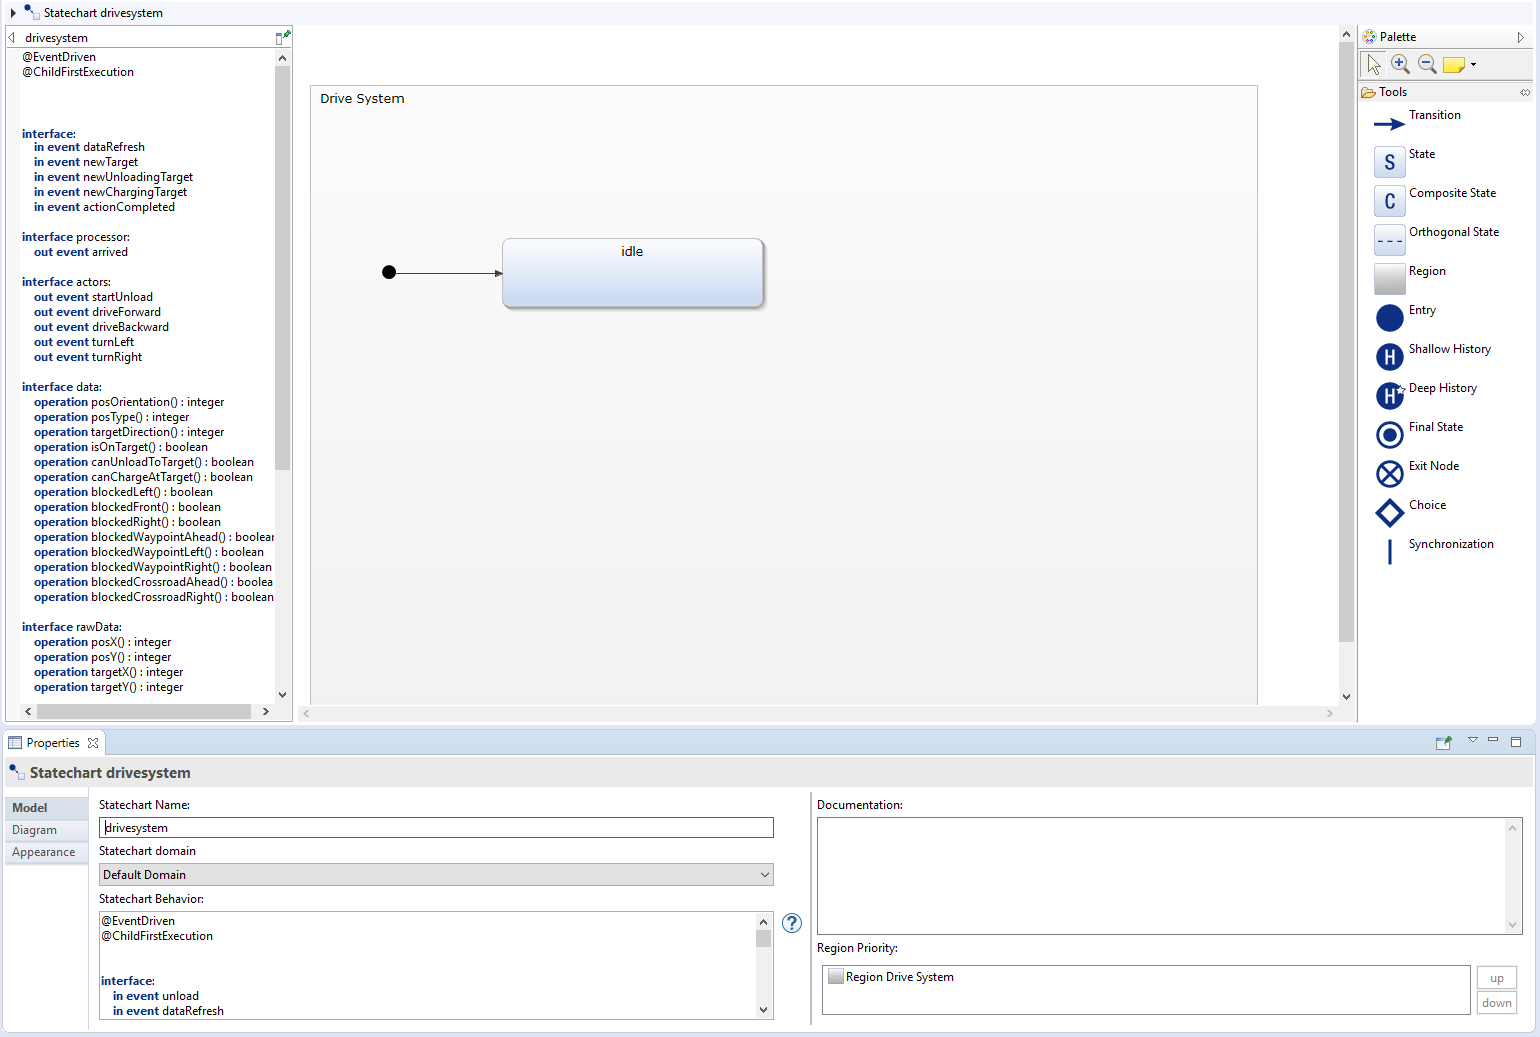
\includegraphics[width=1\textwidth]{yakindu_fenster}
	\caption{Die Modellierungsansicht in YAKINDU SCT}
	\label{fig:yakindu_ui}
\end{figure}

Das im \docProjectTitle{} zu modellierende Statechart befindet sich im Ordner \texttt{model}. 
Per Doppelklick auf die entsprechende Datei \texttt{infinitewarehouse\_drivesystem.sct} (oder auf eine andere .sct-Datei) öffnet sich die Modellierungsansicht.

Sollte sich die Modellierungansicht nicht wie erwartet öffnen, muss die aktuell gewählte Perspektive überprüft werden (kleine Icons oben rechts). 
Hier ist \enquote{SC Modeling} auszuwählen. 


\subsubsection{Überblick}
 
Die Modellierungsansicht (siehe \autoref{fig:yakindu_ui}) ist wie folgt strukturiert:

\begin{itemize}
	\setlength\topsep{-1em}
	\setlength\itemsep{-0.5em}
	\item In der Bildschirmmitte befindet sich das eigentliche Statechart-Diagramm.
	\item Auf der linken Seite befindet sich der Definitionsbereich des Statecharts, der dem Klassendiagramm aus dem Entwurfsdokument (siehe Abbildung 5 dort) entspricht. 
	Dieser Definitionsbereich darf nicht verändert werden und dient lediglich als Referenz. 
	Interne Ereignisse und Variablen (gekennzeichnet durch das Schlüsselwort \enquote{internal}) dürfen allerdings ergänzt werden.
	\item Auf der rechten Seite befindet sich die Palette mit den Diagrammelementen, die zur Modellierung genutzt werden können. 
	Besonders wichtig sind hierbei die Elemente \enquote{State} (um einen neuen Zustand anzulegen), \enquote{Transition} (um eine Transition zwischen zwei Elementen einzufügen) und \enquote{Choice} (um eine Entscheidung zu definieren).
	\item Im unteren Bereich befindet sich das \enquote{Properties}-Fenster, in dem Eigenschaften des aktuell ausgewählten Elements zu finden sind.
\end{itemize}


\enlargethispage{2\baselineskip}

\subsubsection{Syntax und Konventionen}

Für das Statechart ist die aus der Vorlesung bekannte Syntax zu verwenden.

Zusätzlich gelten einige Konventionen bei der Benennung der Zustände und Regionen. 
Das sollte dem Framework ermöglichen den aktuellen Zustand des Statecharts anzuzeigen:
\begin{itemize}
	\setlength\topsep{-1em}
	\setlength\itemsep{-0.5em}
	\item Die äußerste Region muss \enquote{\texttt{Drive System}} heißen.
	\item Wenn bei der Modellierung (abgesehen von der äußersten Region) weitere Regionen verwendet werden, müssen diese entweder unbenannt sein oder deren Namen müssen mit einem Unterstrich (\enquote{\texttt{\_}}) beginnen. 
	Die Regionnamen dürfen keine Leerzeichen und keine weiteren Unterstriche enthalten.
	\item In Zustandsnamen dürfen keine Unterstriche benutzt werden.
\end{itemize}



\subsubsection{Modellierung von Reaktionen}

Mittels Doppelklick auf den unteren Bereich eines Zustandes öffnet sich ein Textfeld, in dem lokale Reaktionen (z.B. mit \enquote{entry} oder \enquote{exit} als Trigger) spezifiziert werden können.
Mittels Doppelklick auf eine Transition öffnet sich ein Textfeld, in dem auch eine Reaktion spezifiziert werden kann. 

Die Trigger einer Reaktion können jeweils direkt angegeben werden.
Nach den Triggern können Guards in eckigen Klammern definiert werden.
Innerhalb eines Guards können Operationen und Variablen aus dem Definitionsbereich verwendet werden. 

\begin{center}
	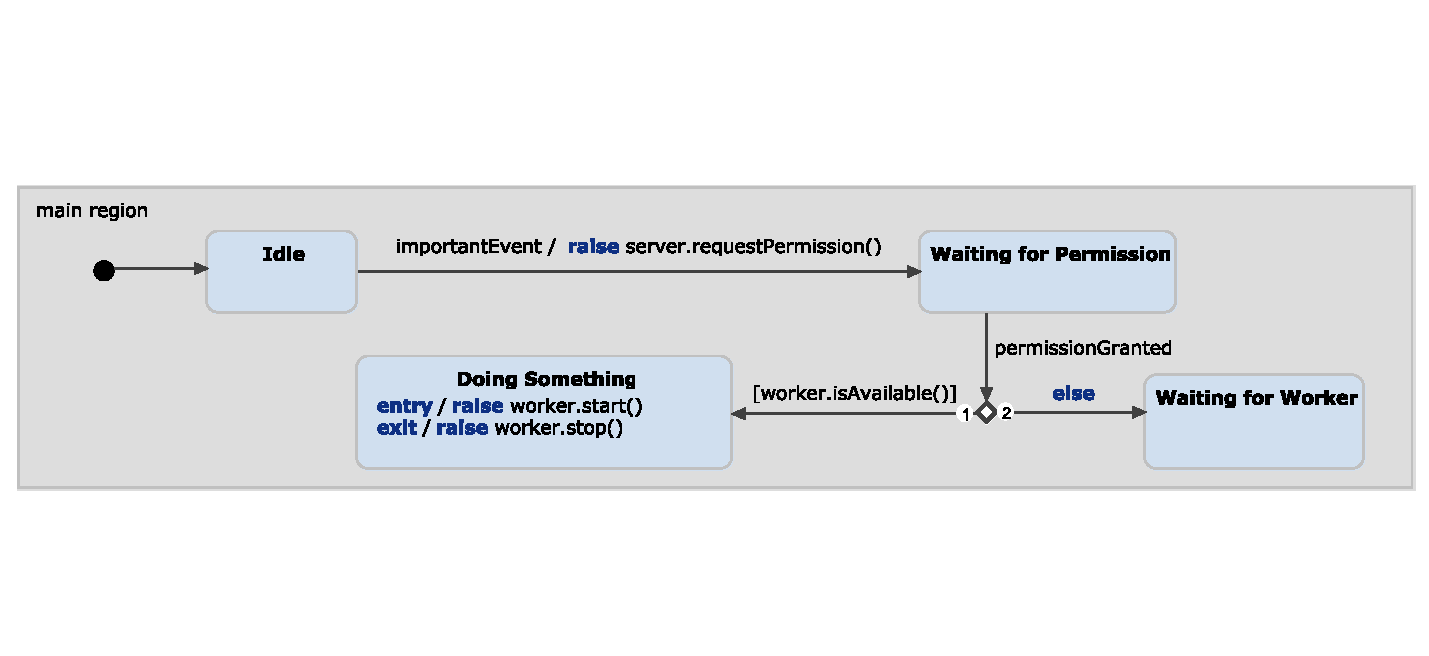
\includegraphics[width=\textwidth]{yakindu_reaktionen}	
\end{center}

Die Effekte sind durch ein \enquote{\texttt{/}} von Triggern und Guards zu trennen. 
Hier können unter anderem ausgehende oder interne Ereignisse genutzt werden, die mit dem Schlüsselwort \enquote{raise} eingeleitet werden.
 
Aus einer Entscheidung oder einem Zustand ausgehende Transitionen sind jeweils nummeriert. 
Die Zahlen geben dabei die Reihenfolge an, in der die Transitionen ausgewertet werden.
Es wird also zuerst die Transition mit der Priorität~1 ausgewertet. 
Wenn die Transition eine Bedingung hat und diese Bedingung wahr ist, werden die Effekte dieser Transition ausgeführt, ansonsten wird die Transition mit der nächsthöchsten Priorität ausgewertet.
Die Prioritäten der ausgehenden Transitionen können im \enquote{Properties}-Fenster einer Entscheidung oder eines Zustandes angepasst werden.


\subsubsection{Subdiagramme}
Um das Statechart übersichtlich zu halten, ist es möglich Subdiagramme anzulegen. 
Dazu kann ein beliebiger Zustand rechts angeklickt und dann \enquote{Create Subdiagramm} ausgewählt werden, um den Zustand mit einem Subdiagramm zu versehen. 
Solcher Zustand ist dann mit einem kleinen Icon unten rechts markiert. 
%Dieses Icon kann angeklickt werden, um das Subdiagramm zu öffnen.
Statt eines Zustandes mit Subdiagramm kann auch ein hierarchischer Zustand genutzt werden.

Ein Zustand mit Subdiagramm bzw. ein hierarchischer Zustand muss genau eine ausgehende Transition ohne Trigger haben. 

\begin{center}
	\raisebox{-\height}{
		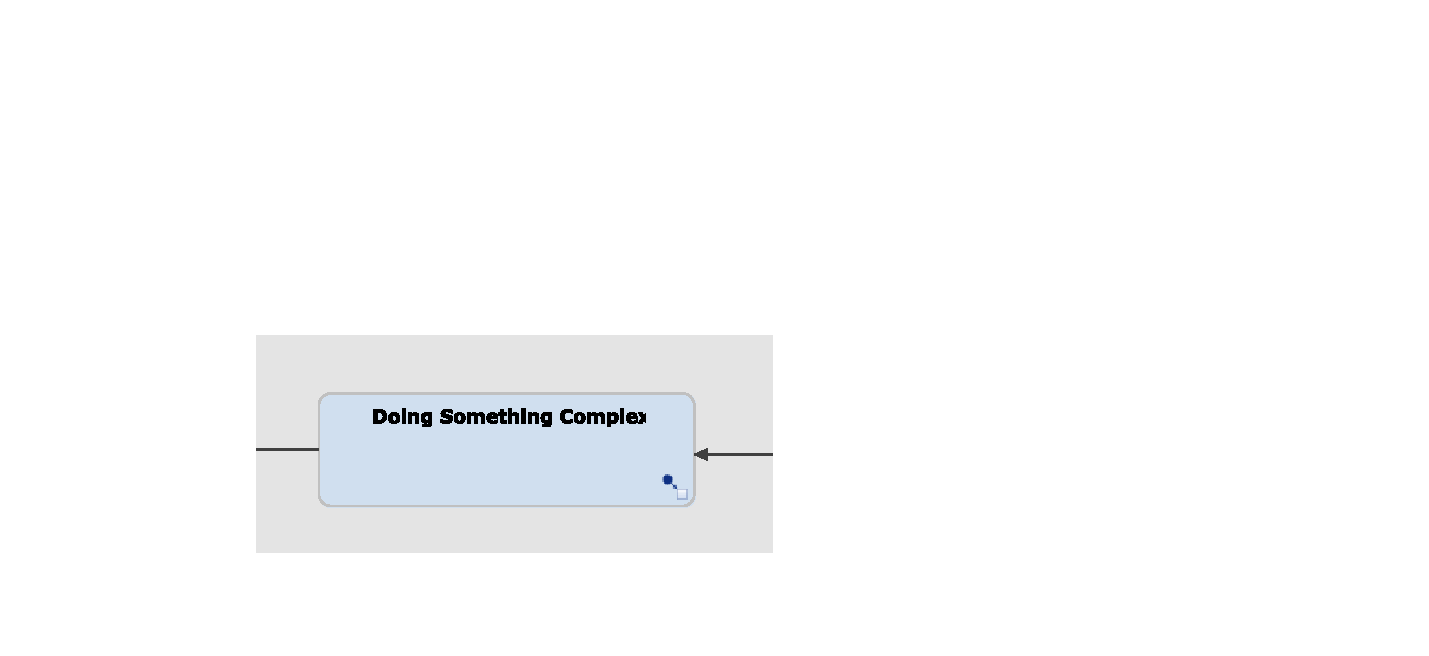
\includegraphics[scale=0.6]{yakindu_subdiagram_extern}	
	}
	~~~~~~~~~~~
	\raisebox{-\height}{
		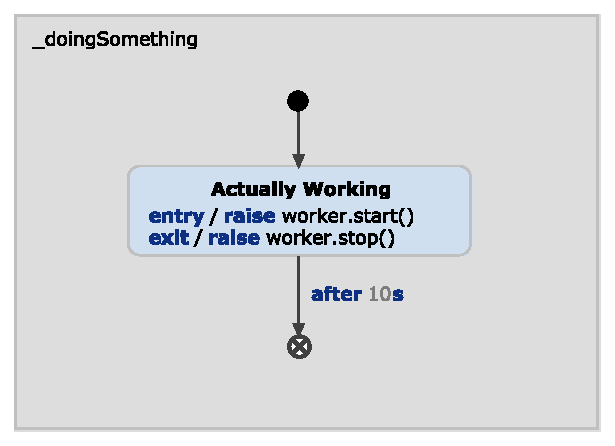
\includegraphics[scale=0.6]{yakindu_subdiagram_intern}	
	}
\end{center}
 
Durch einen Klick auf das Icon in der rechten unteren Ecke eines solchen Zustandes wird das Subdiagramm in einem neuen Tab geöffnet. 
Hier muss zuerst eine neue Region angelegt werden. 
Innerhalb dieser Region kann nun frei modelliert werden (insbesondere können mehrere Subdiagramme ineinander geschachtelt werden).
Dabei muss beachtet werden, dass es innerhalb der angelegten Region ein \enquote{Entry} sowie einen \enquote{Exit Node} geben muss (nicht zu verwechseln mit dem \enquote{Final State}). 
Nachdem das Subdiagramm diesen \enquote{Exit Node} erreicht hat, wird die Behandlung des äußeren Diagramms entlang der triggerlosen Kante fortgesetzt.




%%%%%%%%%%%%%%%%%%%%%%%%%%%%%%%%%%%%%%%%%%%%%%%%%%%%%%%%%%%%%%%%%%%%%%%%%%%%%%%%%%%%%%%%%%%%
 



\subsection{Simulation}

Das Simulationsfeature von YAKINDU SCT ermöglicht ein manuelles Simulieren und Testen des Statecharts. 
Man startet die Simulation für die .sct-Datei durch einen Klick auf den \enquote{Run}-Button.

Der Modellierungsbereich wird während einer Simulation durch eine Ansicht ersetzt, in der das Statechart nicht mehr bearbeitet werden kann, aber der aktuelle Zustand bzw. die aktuellen Zustände des Statecharts gelb markiert sind.
Im Simulationsmenü (Tab \enquote{Simulation} rechts) können Trigger ausgelöst sowie die Rückgabewerte von Operationen gesetzt werden.

Eine laufende Simulation kann durch einen Klick auf das rote Rechteck (\enquote{Stop}-Symbol) oben im Simulationsmenü beendet werden.




%%%%%%%%%%%%%%%%%%%%%%%%%%%%%%%%%%%%%%%%%%%%%%%%%%%%%%%%%%%%%%%%%%%%%%%%%%%%%%%%%%%%%%%%%%%%
 



\subsection{Codegenerierung}

Neben der internen Simulation bietet YAKINDU SCT die Möglichkeit, Code aus einem State\-chart zu generieren. 
Dies ermöglicht dann das Einbinden dieses Codes in eine eigene Simulationsumgebung (z.B. in den im \autoref{sec:framework} beschriebenen Validierungsframework).

Zur Codegenerierung muss auf die mitgelieferte Konfigurationsdatei \texttt{infinitewarehouse\_drivesystem.sgen} rechts geklickt und \enquote{Generate Code Artifacts} ausgewählt werden.
Nach der Erfolgsmeldung im Konsolenfenster befindet sich der generierte Quelltext im Ordner \texttt{src-gen}. 
%Die Roboter verhalten sich dann im Simulator entsprechend dem zuletzt generierten Code.

\enlargethispage{1\baselineskip}




%%%%%%%%%%%%%%%%%%%%%%%%%%%%%%%%%%%%%%%%%%%%%%%%%%%%%%%%%%%%%%%%%%%%%%%%%%%%%%%%%%%%%%%%%%%%
 


 

\subsection{Bekannte Probleme}

In seltenen Fällen reagiert die Modellierungsansicht von YAKINDU SCT nicht mehr auf alle Mausklicks und Tastendrücke (z.B. auf die \enquote{Entf}-Taste).
Um dies zu beheben, genügt es die .sct-Datei zu schließen und erneut zu öffnen.

	\newpage
	%!TEX root = ../toolhinweise.tex

\section{Nutzung des Validierungsframeworks}
\label{sec:framework}

\enlargethispage{1\baselineskip}

\begin{figure}[t]
	\centering
	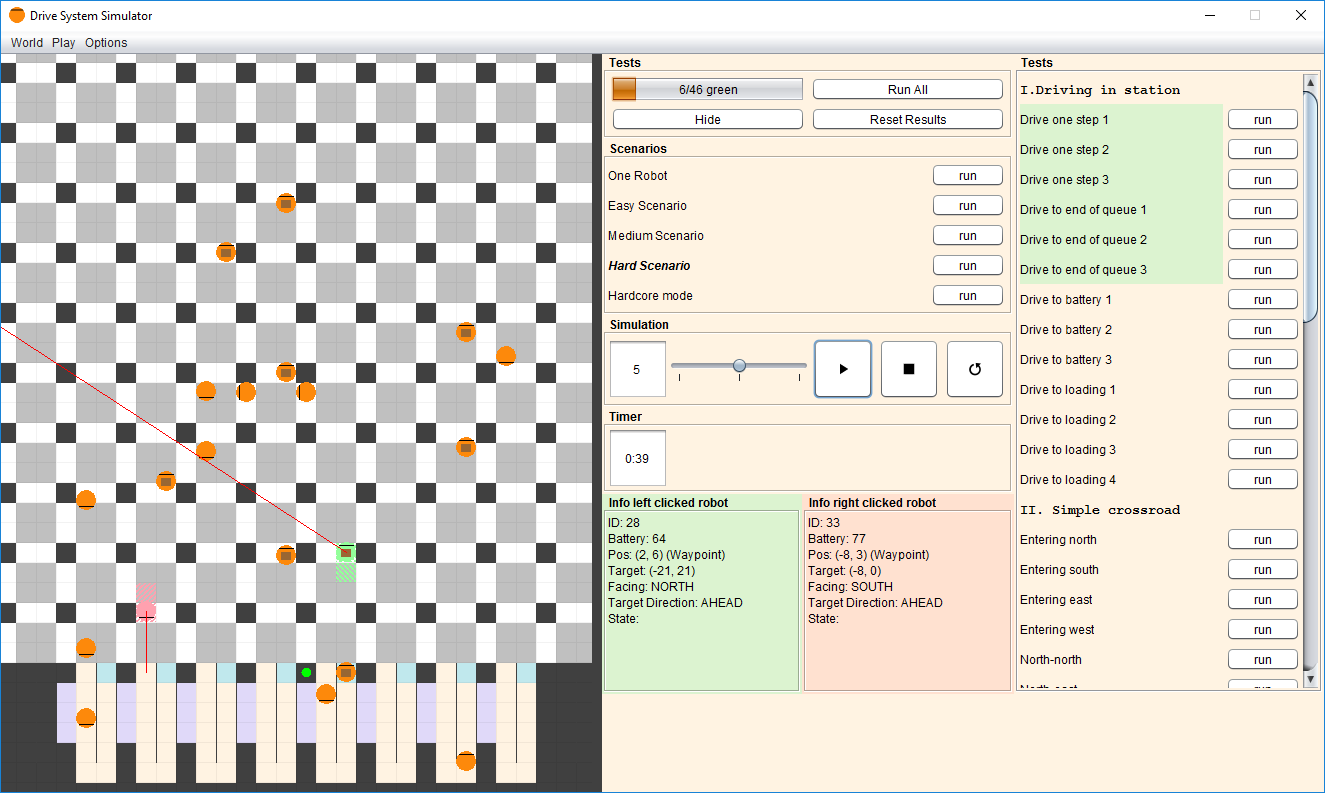
\includegraphics[width=1\textwidth]{simulator_fenster}
	\caption{Das für das \docProjectTitle{} gegebene Validierungsframework.}
	\label{fig:framework_ui}
\end{figure}


Das Validierungsframework kann gestartet werden, indem im \enquote{\red{PROJEKTNAME}}-Projekt die Datei \texttt{App.java} unter \texttt{src/de.hpi.mod.sim} ausgeführt wird. 
Dazu muss die Datei mit einem Rechtsklick angeklickt werden und im Menü \enquote{Run as} $\rightarrow$ \enquote{Java Application} ausgewählt werden. 
Für das wiederholte Ausführen ist \texttt{App.java} dann auch in der Toolbar im \enquote{Run}-Menü hinterlegt.
 
\subsection{Fenster}

Das Framework öffnet sich in einem neuen Fenster (siehe \autoref{fig:framework_ui}).
Das Fenster ist unterteilt in die \nameref{subsec:simulation} links, verschiedene Menüoptionen zum Festlegen von \nameref{subsec:settings} und Starten von \nameref{subsec:scenarios} in der Mitte sowie eine Liste an \nameref{subsec:tests} rechts.  


\subsection{Simulationsfläche}
\label{subsec:simulation}

Die Simulationsfläche bildet eine Paketsortieranlage ab, deren Struktur im Entwurfsdokument genauer beschrieben ist. 
Auf dieser Fläche bewegen sich die simulierten Roboter.

Die Größe der Simulationsfläche (und damit die Anzahl der simulierten Roboter) hängt von der Fenstergröße ab. 
Dementsprechend kann die Fenstergröße nur verändert werden, wenn gerade keine Simulation läuft.

Zur Navigation auf der Simulationsfläche können die Pfeiltasten verwendet werden.
Mit der Tastenkombination aus \enquote{Strg} und \enquote{+} bzw. \enquote{-} kann hinein- bzw. hinausgezoomt werden.


\subsection{Einstellungen}
\label{subsec:settings}

Im mittleren Teil des Fensters sind alle wichtigen Einstellungen zu finden.

Diese befinden sich insbesondere im Bereich \enquote{Simulation}. 
Dort kann per Schieberegler die Geschwindigkeit der Simulation eingestellt werden. 
Mit den benachbarten Schaltflächen kann das aktuell laufende Szenario bzw. Test pausiert, gestoppt oder neu gestartet werden. 
Zum Pausieren und Fortfahren kann auch die Leertaste verwendet werden.

Während eines laufenden Szenarios oder Tests können auf der Simulationsfläche einzelne Roboter angeklickt werden. 
Die Informationen des zuletzt mit links bzw. rechts angeklickten Roboters werden im unteren Bereich dargestellt.


\subsection{Szenarien}
\label{subsec:scenarios}

Im Bereich \enquote{Scenarios} (mitte oben) kann Simulation eines Szenarios gestartet werden. 
Je nach gewähltem Szenario, werden dabei ein oder mehrere Roboter auf der Simulationsfläche platziert.
Diese Roboter werden durch die aktuelle Version des generierten Codes gesteuert. 
Es werden kontinuierlich Aufträge an die Roboter übermittelt, bis das Szenario beendet wird. 
Kollisionen und Deadlocks führen zum vorzeitigen Abbruch des Szenarios.

Das aktuell ausgewählte Szenario ist durch eine Hervorhebung des Namens markiert.


\subsection{Tests}
\label{subsec:tests}


Ein Test prüft eine vordefinierte Fahrsituation und gibt unmittelbar eine Rückmeldung über deren Erfolg. 
Das Verhalten der Roboter kann dabei auf der Simulationsfläche beobachtet werden.

Für die Steuerung der Tests gibt es den Bereich \enquote{Tests} im mittleren Teil des Fensters sowie die Liste aller Tests im rechten Teil des Fensters. 
Die Liste aller Tests kann mit einem Klick auf \enquote{Hide} bzw. \enquote{Show} aus- bzw. eingeblendet werden.

Jeder Test kann individuell über \enquote{Run} gestartet werden. 
Alternativ kann per \enquote{Run All} die gesamte Testliste automatisch abgearbeitet werden.

Die Farbe, mit der der Titel eines Tests hinterlegt wird, gibt Auskunft über den Erfolg bzw. den Misserfolg dieses Tests beim letzten versuchten Durchlauf. 
Einen Überblick über die Testergebnisse gibt zudem der Fortschrittsbalken im Bereich \enquote{Tests}. 
Die Testergebnisse bleiben auch nach dem Schließen des Simulators erhalten, damit nicht jedes Mal die gesamte Testliste neu geprüft werden muss. 
Die Testergebnisse können mittels \enquote{Reset Results} gelöscht werden.



\end{document}










